\paragraph{Example}
 	\begin{center}
 		\includegraphics[width=\linewidth]{./lect12/pic1.png}
 	\end{center}
 	
 	\paragraph{Velocity of mass center}
 	
 $$	\dot{\vec{R}}_{cm} = \frac{\sum{\dot{\vec{r}}_i m_i}}{\sum m_i} = \frac{\sum \vec{v}_i m_i}{\sum m_i}$$
 \paragraph{Acceleration of mass center}
 $$	\sum{m_i}\ddot{\vec{R}}_{cm} = \sum{\ddot{\vec{r}}_i m_i} = \sum \vec{F}_i$$
 
 Or:
 
 $$\underbrace{M_{total} }_{\parbox{2cm}{\centering \scriptsize total mass ($\sum m_i$)}} \cdot \ddot{\vec{R}}_{ct} = \underbrace{\sum \vec{F}_i}_{\parbox{2cm}{\centering \scriptsize sum of forces on particles}} \stackrel{3rd \: law}{=} \vec{F}_{external}$$
 
 \paragraph{System of center of mass}
 	\begin{center}
 	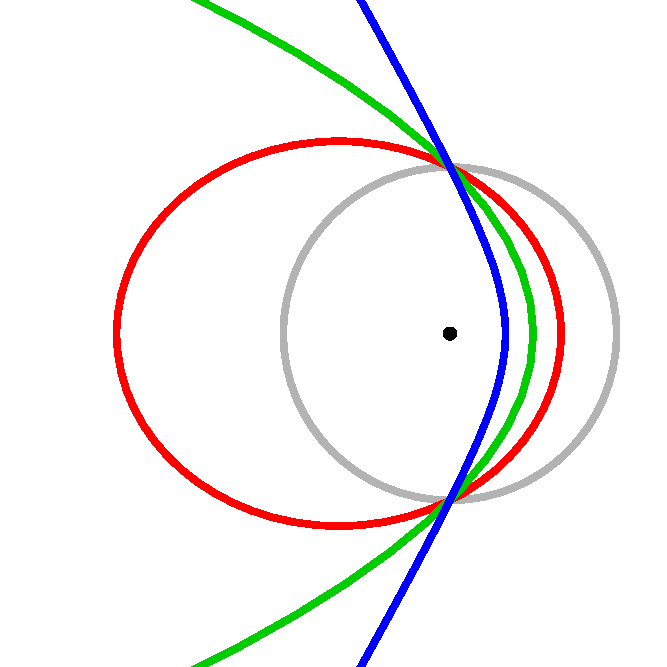
\includegraphics[width=\linewidth]{./lect12/pic2.png}
 \end{center}
 
 $$\vec{r}_{icm} = \vec{r}_i - \vec{R}_{cm}$$
 
 Then impulse of center of mass relative to its own system is
 
 $$\vec{p}_{cm\:to\:cm} = \sum p_{icm} = \sum \dot{\vec{r}}_{icm} m_i$$
 
 $$\vec{p}_{cm\:to\:cm}  = \sum \left( \dot{\vec{r}}_i - \dot{\vec{R}}_{cm}\right) m_i = \sum \vec{v}_i m_i - \dot{vec{R}}_{cm} \sum m_i = 0$$
 
 \paragraph{Example} Mass of $m_1=0.4kg$ moves with $v_1 = 6 \frac{m}{s}$ and collides with mass $m_2=0.1kg$ in rest. From conservations of impulse and energy:
 $$m_1v_{10}+m_2v_{20} = m_1v_1+m_2v_2$$ 
 $$\frac{1}{2}m_1v^2_{10}+\frac{1}{2}m_2v^2_{20} = \frac{1}{2}m_1v^2_1+\frac{1}{2}m_2v^2_2$$ 
 
 \begin{enumerate}
 	\item First solution is trivial: $v_1=6 ms^{-1}$ and $v_2 = 0 ms^{-1}$, but isn't interesting.
 	\item Second solution is $v_1=3.6 ms^{-1}$ and $v_2 =9.6 ms^{-1}$.
 \end{enumerate}
 
 Velocity of mass center before collision:
 
 $$\vec{v}_{cm} = \frac{\vec{v}_{10} m_1 + \vec{v}_{20} m_2 }{m_1+m_2} = 4.8 ms^{-1}$$
 
 And after:

$$\vec{v}_{cm} = \frac{\vec{v}_{1} m_1 + \vec{v}_{2} m_2 }{m_1+m_2} = 4.8 ms^{-1}$$

Impulse of system before and after is:

$\vec{p} = m_1 (\vec{v}_1 - \vec{cm}) + m_2(\vec{v}_2 -\vec{v}_{cm})= 0$

Relative to center of mass:

$$\vec{v}_{10cm} = \vec{v}_{10}-\vec{cm}= 1.2 ms^{-1} \quad \vec{v}_{20cm} = \vec{v}_{20}-\vec{cm}= -4.8 ms^{-1}$$

$$\vec{v}_{1cm} = \vec{v}_{1}-\vec{cm}= -1.2 ms^{-1} \quad \vec{v}_{2cm} = \vec{v}_{2}-\vec{cm}= 4.8 ms^{-1}$$

\paragraph{Example}


\paragraph{System of center of mass}
\begin{center}
	\includegraphics[width=0.2\linewidth]{./lect12/pic3.png}
\end{center}

Two balls, heavy and light are falling with same velocity. What happens?

\begin{enumerate}
	\item Heavy ball collides with floor. Effectively center of mass of ball and floor is the floor, so it returns with same speed and opposite direction.
	\item Now light ball collides with heavy ball. Similarly, center of mass of two balls is the heavy one, so the light ball returns with the same speed relative to heavy ball and opposite direction. However, relative to the floor, the speed is triple, since the big ball has a velocity relative to the floor.
\end{enumerate}

If we have more than one ball, the process returns on itself couple of times.

This effect is used in gravitational slingshot:


\begin{center}	
	\includesvg[eps,svgpath = lect12/,width=0.75\linewidth]{pic4}
\end{center}

Here instead of collision we use gravitational force.

\paragraph{Collision of two bodies in 3D}
For two bodies collision happens in plane formed by two vectors of speed. We have total of 4 variables: $v_1, \theta_1, v_2, \theta_2$ or $v_{1x}, v_{1y}, v_{2x}, v_{2y}$. This is elastic collision i.e. kinetic energy is conserved. There are only three equations: conservation of impulse for each of axis and conservation of energy. So to acquire full solution we need some new factor. 

\begin{center}
	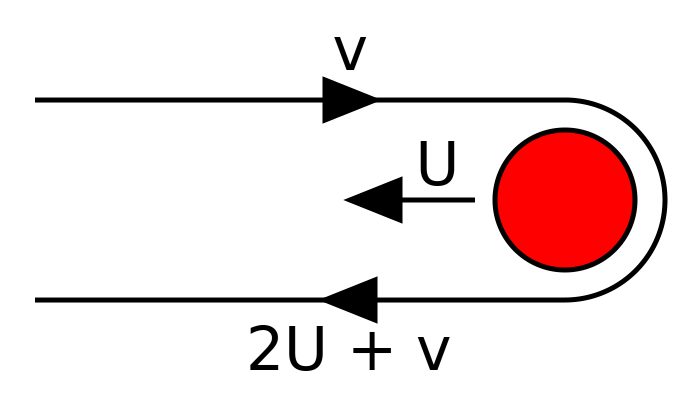
\includegraphics[width=\linewidth]{./lect12/pic4.png}
\end{center}